\documentclass[12pt]{report}
\usepackage[utf8]{inputenc}
\usepackage[main=russian,english]{babel}
\usepackage[left=20mm, top=15mm, right=20mm, bottom=10mm, nohead, nofoot]{geometry}

\usepackage{graphicx}
\usepackage{caption}
\usepackage{wrapfig}
\usepackage{multicol}
\usepackage{lipsum}
\usepackage{mwe}
\usepackage{enumerate}

%\usepackage{listings}
%\lstloadlanguages{java}


% -----------------------------------
%
% !!! Сделать нормальное содержание и ссылки !!!
%
% -----------------------------------

% \def \var {value}
\newcommand{\ReportTheme}{Практика}
\newcommand{\ReportAuthor}{Данилевич Леонид, Лельчук Александр, 2022А класс}

\title{\bf \ReportTheme}
\author{\it \ReportAuthor}
\date{\today}

% 1. Титульный лист. (Одинаковая по форме. Взять в нетскуле)
% 2. Аннотация. (Около абзаца. Кратко, какая поставлена задача, какой результат получен. Делается в последний момент)
% 3. Оглавление.
% 4. Введение. (Где родилась задача. Ваша задача - подспорье в решении какой-то более глобальной. Зачем это всё нужно = Обоснование работы)
% 5. Постановка задачи. Сформулировать задачу так, чтобы можно было её решить математически/померить экспериментально/и т д.
% 6. Методика разрешения задачи. Как решается задача: математически/экспериментально/программно и т д. Подробности. С помощью каких механизмов.
% 7. Результаты. Что вы померили/насчитали/
% 8. Анализ результатов. Что означают результаты. Совпадают ли с предсказаниями. Что следует из результатов.
% 9. Список литературы. На что вы опирались.
% 10. Благодарности. С кем вы работали, кто вас консультировал, кто помогал и т п.

%\usepackage{mathptmx}

\begin{document}
   % \maketitle
   % титульный лист

    \begin{center}
    \large { {\bf Лицей «Физико-техническая школа»  Санкт-Петербургского Академического университета   } } 
    
    \vspace*{6\baselineskip}
    
    \vfill
    \large { {\bf Курсовая работа (отчет по практике) } } 
    
    \vspace*{6\baselineskip}
    
    Создание программы генериующей кроссворды из регулярных выражений \\
    \vspace*{3\baselineskip}
    
    \end{center}        
    \begin{flushright}
        Работу выполнили: \\
        Данилевич Леонид (2022А) \\
        Лельчук Александр (2022А) \\
        Научный руководитель: \\
        Дворкин Михаил Эдуардович \\
        Место прохождения практики: \\
        Лицей <<ФТШ>>
    \end{flushright}
    \vspace*{5\baselineskip}
    \begin{center}
        Санкт-Петербург, 2021
    \end{center}        
%----------------------------------------------------------------------------------------------------------
    \newpage % Аннотация
    \chapter*{Аннотация}
     Мы смогли разработать алгоритм генерации строк, которые подходят под различне человекочитаемые паттерны (например: палиндромы, прогресии, словарные ключи, повторы и так далее), которые могли бы легко восприниматься человеком.
     Также мы смогли создать уникальный алгоритм генерации наиболее короткого регулярного выражения для задданной строки.

    
%----------------------------------------------------------------------------------------------------------
    \newpage % Оглавление
\renewcommand*\contentsname{Кроссворды из регулярных выражений }
\tableofcontents
%----------------------------------------------------------------------------------------------------------
    \newpage % Введение
\chapter{Введение}
Регулярные выражения — формальный язык поиска подстрок в тексте и манипуляций с ними. Например, регулярному выражению «.*amp(le)?» соответствуют строки «Sample», «example», «lamp» и некоторые другие. С помощью регулярных выражений можно достаточно легко искать в тексте подстроки определённого формата и заменять их на соответствующие им другие подстроки. В 2013 году, как задание конкурса «MIT Mystery Hunt», был создан кроссворд из регулярных выражений (рис. \ref{pic:MITHex}). Мы решили написать приложение, автоматически генерирующее подобные кроссворды, а также позволяющее их решать. Мы считаем, что такое приложение будет полезно многим людям, изучающим регулярные выражения, а для уже знакомых с ними оно будет просто интересно.
 \begin{figure*}[ht!]
 \centering
    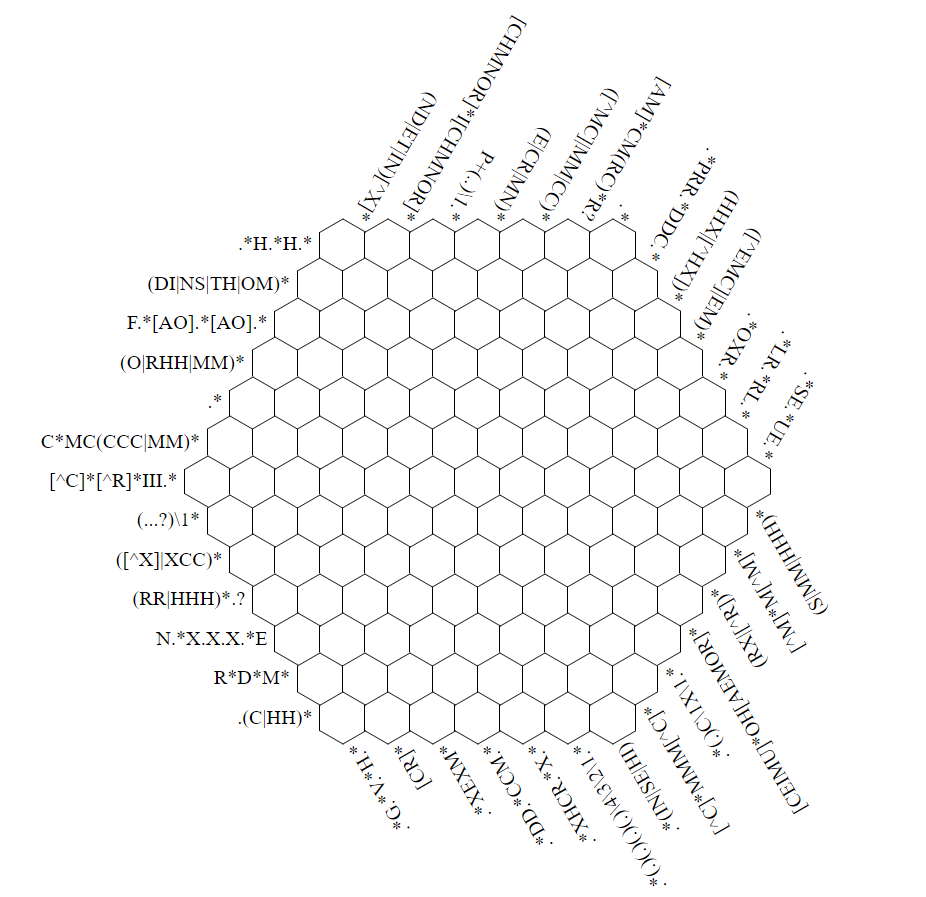
\includegraphics[width=.7\textwidth]{MITHexagon.png}
    \caption{\label{pic:MITHex}Кроссворд с «MIT Mystery Hunt» 2013 года}
\end{figure*}

%----------------------------------------------------------------------------------------------------------
    \newpage % Постановка задачи
   \chapter{Постановка задачи}
   
   Создать приложение на базе Android, функционалом которого является генерация, отображение и поддержка решения пользователем красивых кроссвордов из регулярных выражений.
   
   Кроссворд из регулярных выражений -- клеточная сетка правильной формы (прямоугольник, шестиугольник и т. д). Решением кроссворда называется такое сопоставление символа каждой клетке, что линии, образованные этими символами (например, в прямоугольнике это столбцы и строчки) формируют буквенные строчки, кодирующиеся соответственными регулярными выражениями.
   
   Мы называем кроссворд из регулярных выражений красивым, если он имеет единственное решение. В нём регулярные выражения, использующиеся для кодирования линий символов, разнообразны (используется большое количество конструкций: символьные классы, группы, перечисления, квантификаторы, обратные ссылки и т. д.). В полученных линиях символов должны наблюдаться паттерны, которые легко воспринимаются человеком.


%----------------------------------------------------------------------------------------------------------
    \newpage % Методика решения задачи
\chapter{Методика решения задачи}

Так как задача состоит в написании программы, то решается программно. Задача дробится на части: 
\section{Программное решение кроссворда}
Собственно, решение уже имеющегося кроссворда. Понадобится для оценки сложности кроссворда и и удостоверения единственности решения.
\subsection{Разбор регулярных выражений} Для решения произвольного кроссворда необходимо разобрать («распарсить») регулярные выражения, кодирующие его строчки. Для этого написана рекурсивная функция с запоминанием ответа (техника «мемоизации» динамического программирования), которая для заданного регулярного выражения и требуемой длины строчки находит в компактном виде всевозможные строчки, подходящие под данное выражение. Компактный вид обусловлен тем, что строчки состоят не из символов, а из битовых масок, где из любой маски можно выбрать любой символ и получить корректную строчку. Обратные ссылки в регулярных выражениях обрабатываются следующей техникой: два символа, запрашиваемые быть одинаковыми, соотвествуют одному и тому же битовому объекту-маске.
\subsection{Отгадывание букв} После разбора регулярных выражений кроссворд решается методом инкрементальных улучшений. Изначально каждой букве сопоставлена битовая маска, соответствующая всем символам алфавита. Алгоритм рассматривает все ещё не разгаданные буквы по порядку, сужая для каждой множество возможных значений. Существует вероятность встретить кроссворд, имеющий решение, но нерешаемый данной техникой. Однако для его разгадывания человеку потребуется долгий и утомительный перебор. Создание таких кроссвордов не входит в нашу задачу. В случае полного разгадывания кроссворда можно утверждать, что его решение существует и единственно.

\section{Генерация буквенного заполнения кроссворда} Для красоты кроссворда необходимо образование строк, подходящих под различные регулярные выражения. Максимизируется красота заполнения — субъективное свойство, включающее в себя регулярность кроссворда. Именно, максимизируется количество и длина входящих в кроссворд подстрок, являющихся шаблонами следующих типов: палиндром (строка, читающаяся одинаково слева направо и справа налево); повтор (строка, состоящая из одинаковой части, повторённой несколько раз); прогрессия (строка, в которой на нечётных (в 1-индексации) местах стоят одинаковые буквы, а на чётных - разные; словарный ключ - существующее английское слово.
\subsection{Имитация отжига} Для генерации случайного поля, максимизирующего потенциальную оценку кроссворда, а именно, разнообразие типов регулярных выражений, разгадка необходимой степени сложности, и субъективная оценка красоты, применён метод имитации отжига («simulated annealing»). Большое количество итераций заменяют одну букву на изначально равномерно случайно сгенерированном поле, после чего в некотором случае изменение принимается, поле обновляется.


\section{Генерация регулярных выражений} Генерация регулярных выражений, лучшим образом задающих получившиеся строчки. Пока не реализована.

\section{Оценка сложности, проверка единственности решения} Оценку сложности и проверку единственности решения планируется осуществлять путём программного решения.
        Сложность решения предполагается оценивать, как усреднённое значение количества итераций, требуемых алгоритму для решения сгенерированного кроссворда при рассмотрении клеток, содержащих неразгаданные буквы, в случайном порядке.
   

%----------------------------------------------------------------------------------------------------------
    \newpage % Результаты
    
\chapter{Результаты}
\section{Программное решение кроссворда}
Получившаяся программа успешно разгадывает кроссворды. При вводе регулярных выражений из кроссворда, упоминавшегося во введении (рис. \ref{pic:MITHex}), программа выдаёт следующее решение (рис. \ref{pic:MITSolution})
\begin{figure*}[ht!]
 \centering
    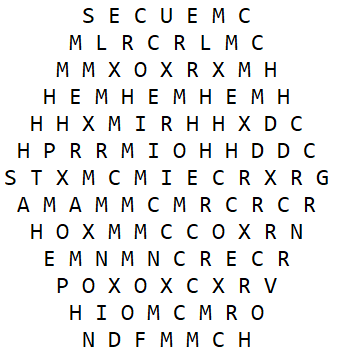
\includegraphics[scale=1.0]{HexagonalOutput1.PNG}
    \caption{\label{pic:MITSolution}Решение кроссворда (рис. \ref{pic:MITHex})}
\end{figure*}
\section{Генерация буквенного заполнения кроссворда}. 
Алгоритм получилось написать. Получились довольно хорошо удовлетворяющие условиям кроссворды (рис. \ref{pic:GenCross}):
\begin{figure*}[ht!]
 \centering
    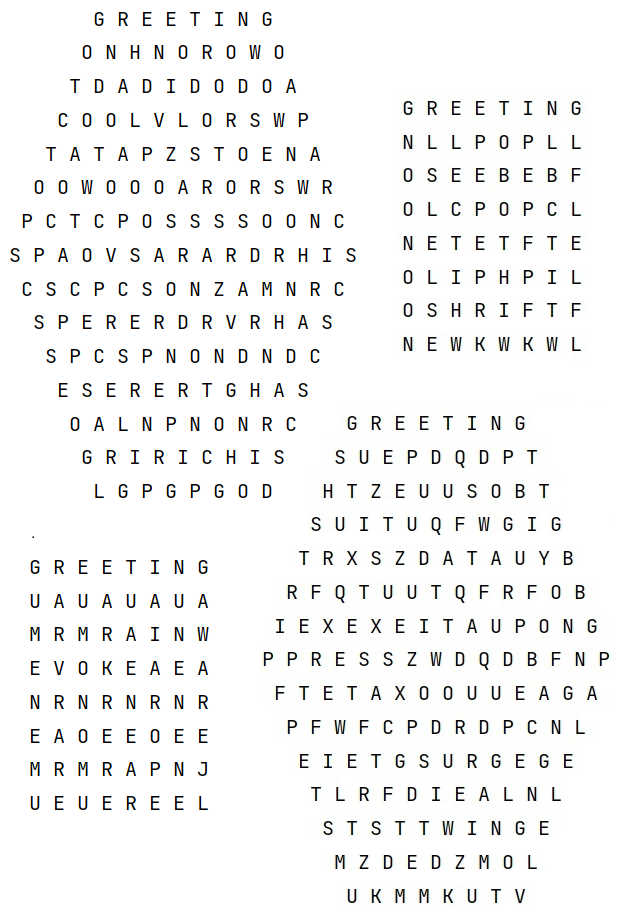
\includegraphics[scale=1.0]{generated8.PNG}
    \caption{\label{pic:GenCross}Сгенерированные кроссворды}
\end{figure*}
Рассмотрим подробнее результат работы отжига. Выделю некоторые существенные паттерны в одном из кроссвордов (рис. \ref{pic:Patterns})
\begin{figure*}[ht!]
 \centering
    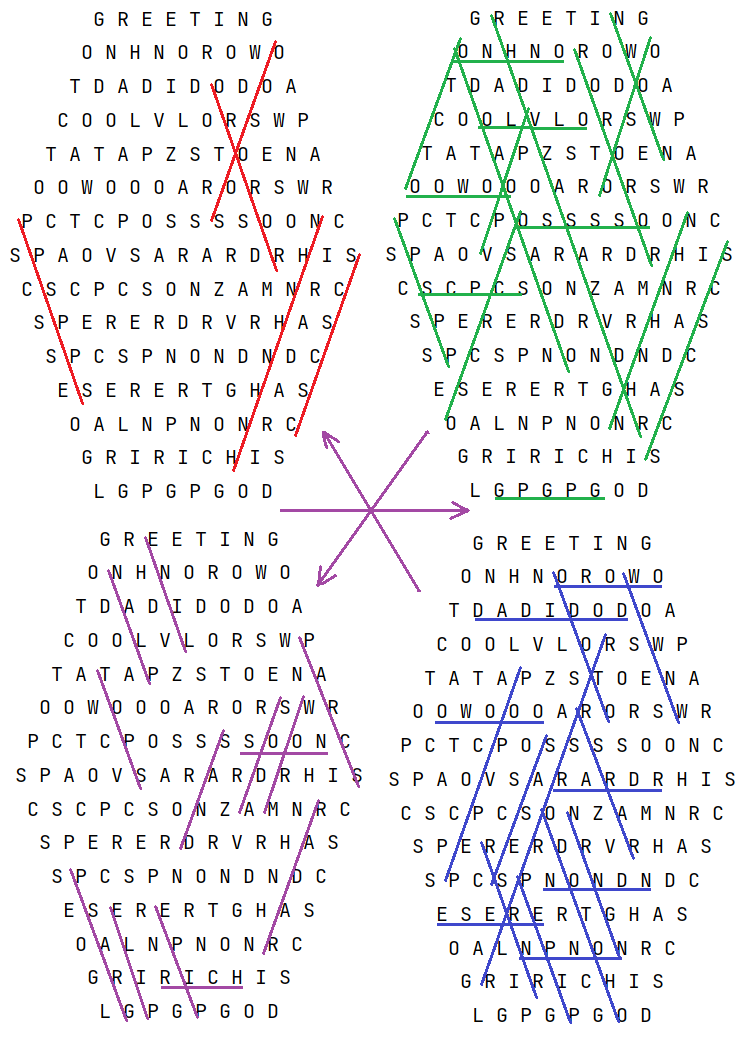
\includegraphics[scale=0.9]{patterns.png}
    \caption{\label{pic:Patterns}Слева направо, сверху вниз: повторы, палиндромы, слова, прогрессии}
\end{figure*}
\section{Генерация регулярных выражений} Генерация регулярных выражений, лучшим образом задающих получившиеся строчки. Пока не реализована.

\section{Оценка сложности, проверка единственности решения} Решение кроссворда заодно проверяет и единственность данного решения. Оценка не реализована, так как оценивать нечего, а именно, по причине отсутствия генерации регулярных выражений. По появлении генерации регулярных выражений сделать оценку будет достаточно просто: лишь слегка модифицировать само решение кроссворда, чтобы помимо решения, оно возвращало усреднённое количество понадобившихся итераций при случайном порядке рассмотрения клеток.

%----------------------------------------------------------------------------------------------------------
    \newpage % Анализ рез-ов    
\chapter{Анализ результатов}
    Пока результаты не очень большие, но мы сделали многое из того, что хотели. \\
    Мы получили новый алгоритм, которого раньше не существовало, и который в перспективе может использоваться не только в нашем приложении, но также для генерации \\
    шаблонов для описания различных строк на основании только лишь одной входной строки. \\

    
%----------------------------------------------------------------------------------------------------------
%    \newpage % Список литры (у нас пуст в общем)

%----------------------------------------------------------------------------------------------------------
    \newpage % Благодарности
\chapter{Благодарности}
Мы благодарим нашего научного руководителя { \bf Дворкина Михаила Эдуардовича } за научное руковождение и направление теоретической части нашей работы.
    \\
    \\
    
    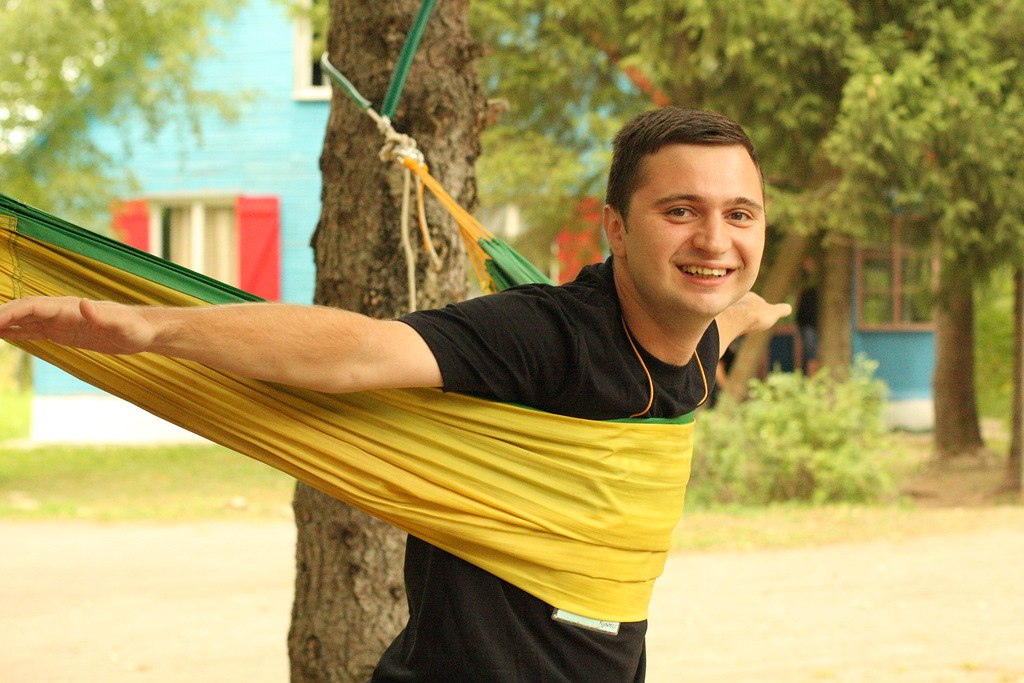
\includegraphics[scale=0.5]{dvorkin2.jpg}\hfill
    

        
\end{document}

